\section{Programmorganisationsplan}
\paragraph{Einleitung}
Im folgenden Abschnitt wird eine Gesamt"ubersicht "uber das Zusammenspiel s"amtlicher Klassen gegeben. Das dazu verwendete UML-Diagram (siehe Abbildung \ref{fig:umlGesamtVereinfacht}, S.  \pageref{fig:umlGesamtVereinfacht}) ist leider relativ gro"s geworden. Falls Sie eine vergr"o"serte Version in ihrem Bildbetrachter sehen m"ochten, folgen Sie bitte dem Link in Lesezeichen"ubersicht des Pdf-Readers. Ansonsten liegt das Bild diesem Projekt auch bei (Name \emph{PP18Vereinfacht.png}). 
\todo{Falls noch Zeit ist, Bild schoener ans Projekt anhaengen}

\embedfilesetup{mimetype=image/png}
\embedfile{programmierhandbuch/Programmorganisationsplan/PP18Vereinfacht.png}

\begin{figure}[b]
	\centering
	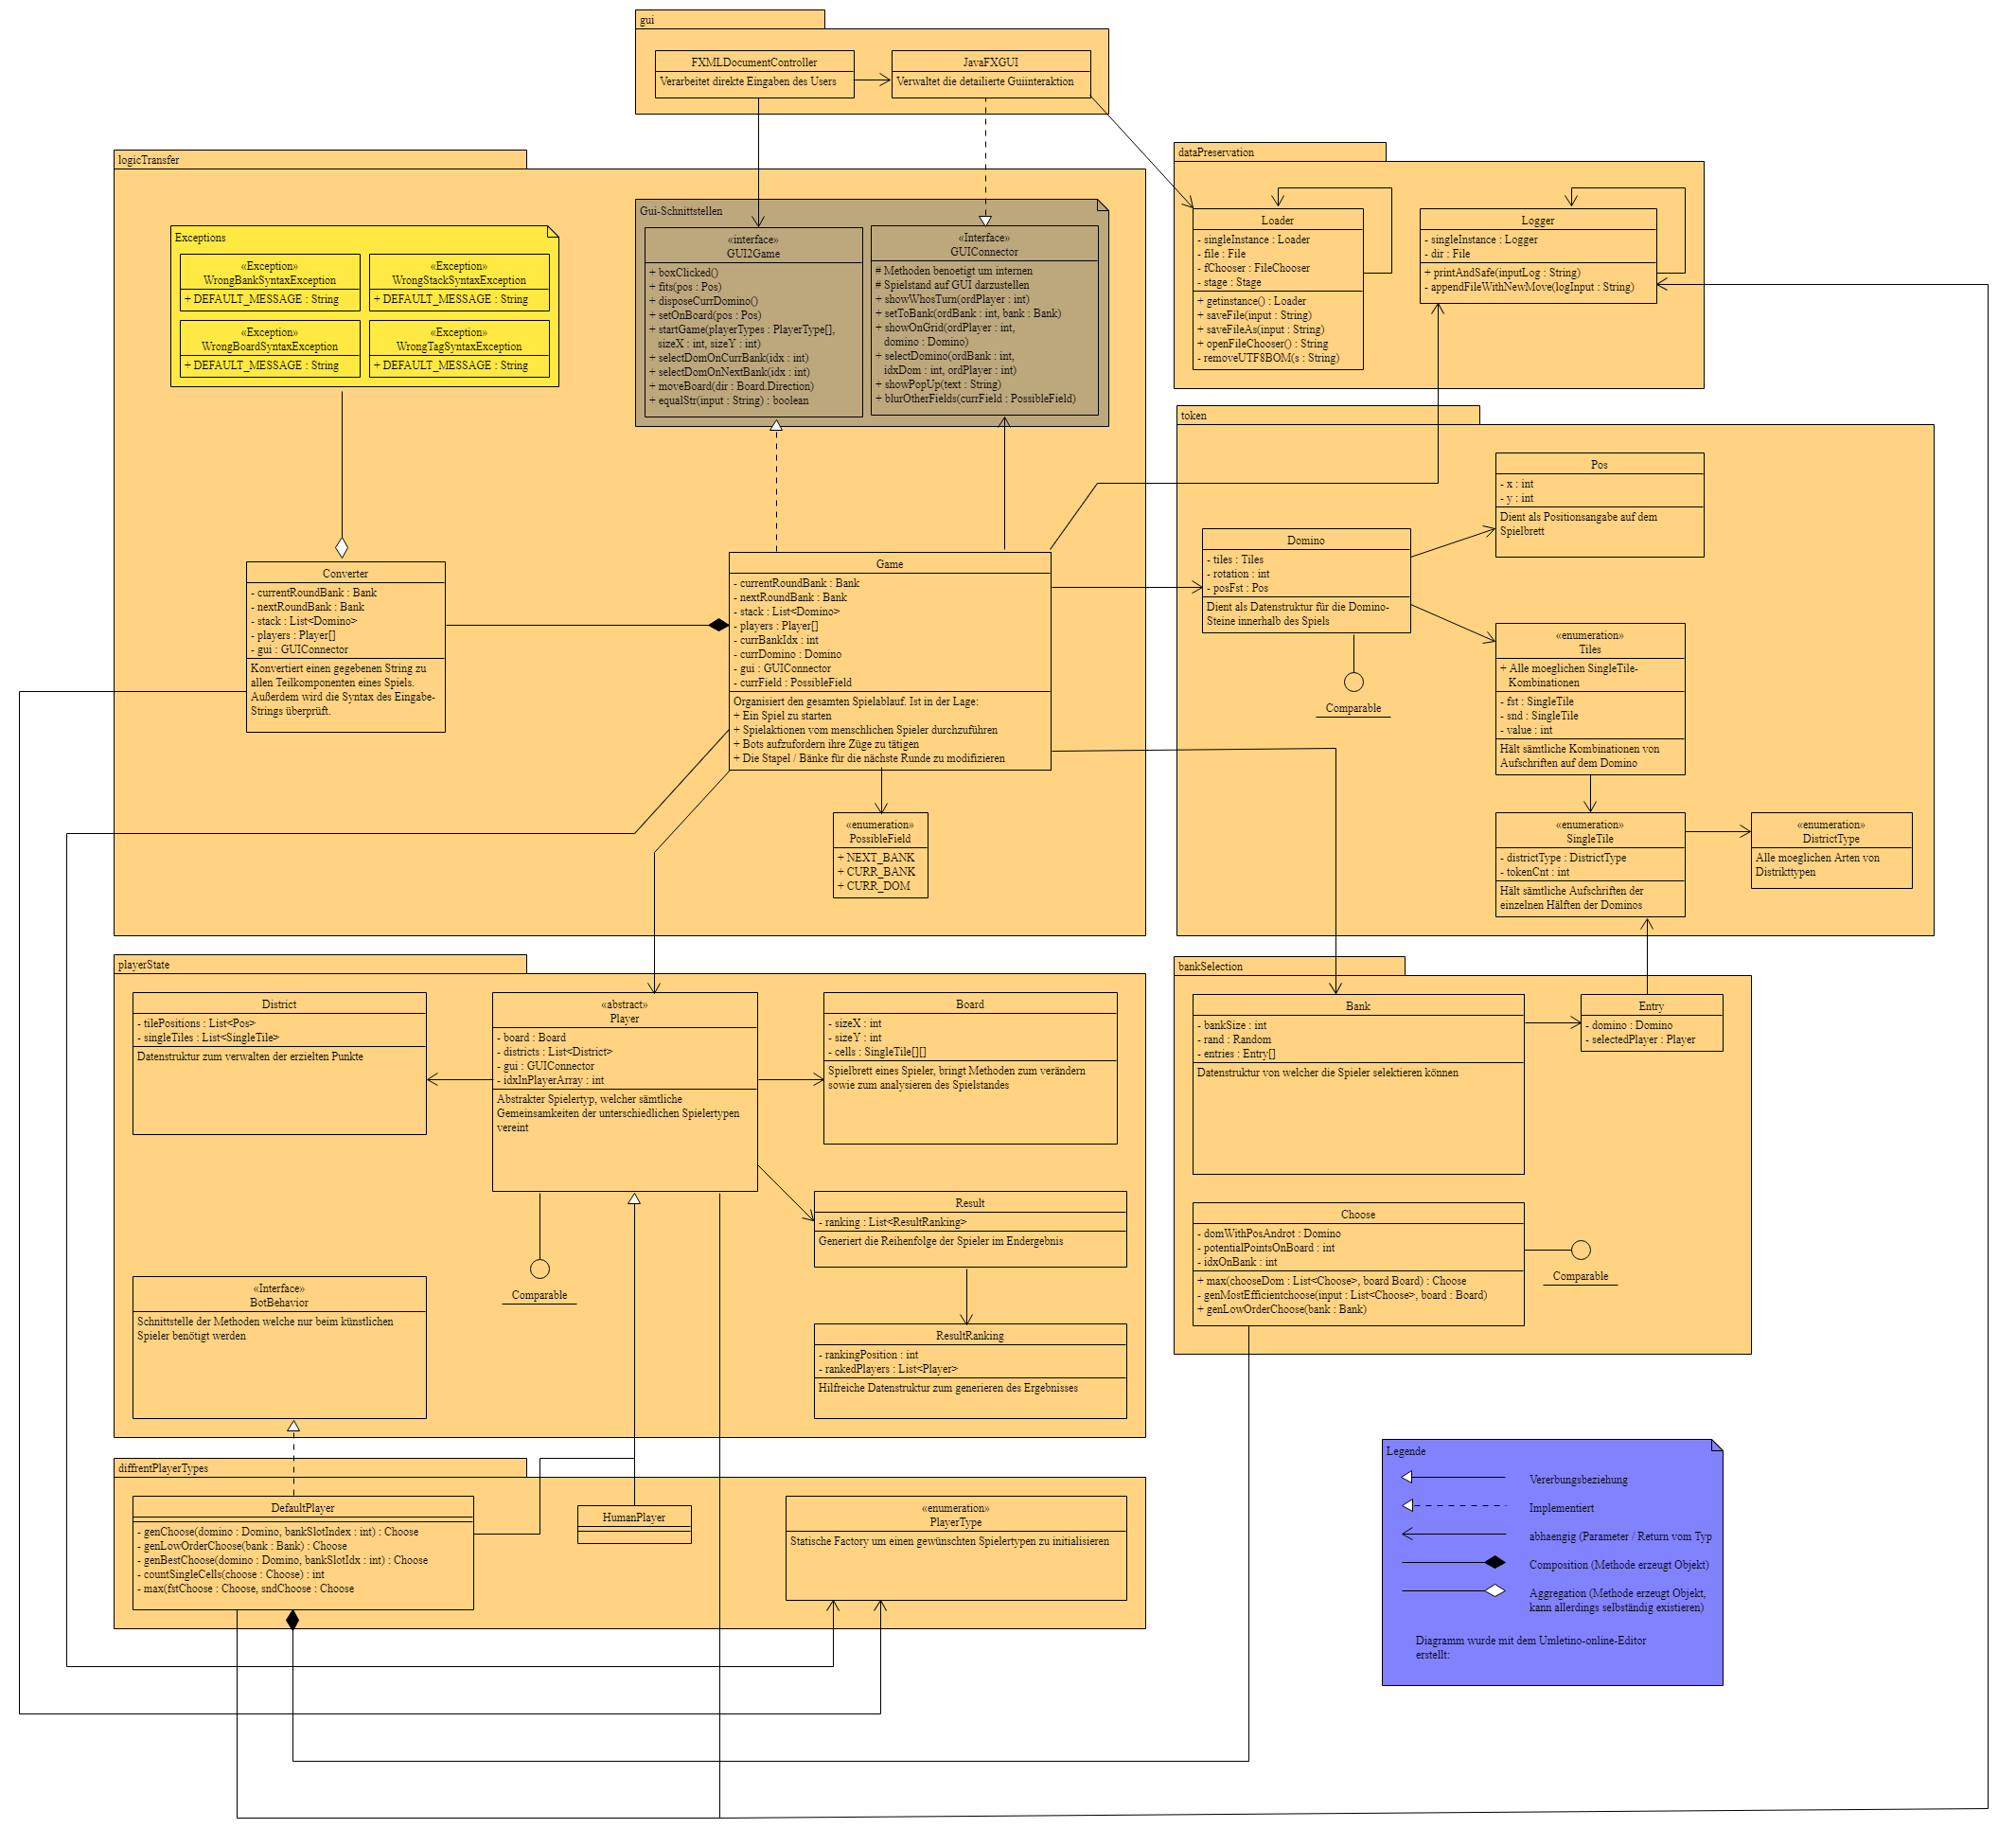
\includegraphics[width=\linewidth]{pics/PP18Vereinfacht}
	\caption{Vereinfachte UML-Darstellung des gesamten Projekts}
	\label{fig:umlGesamtVereinfacht}
\end{figure}